\chapter{REVISIÓN DE LITERATURA}


\textcite{Martin1999}

En este estudio se realizó la evaluación del desempeño de una BCP  con diferentes fracciones de vacío. La bomba de prueba tiene cuatro etapas, con un rotor de 20 mm de diámetro. Los sensores para la medición de presión y temperatura se colocaron en unos dispositivos que se pueden apreciar en la Figura~\ref{fig:Accesorios_montaje_Martin-1999-426}. En la Figura~\ref{fig:arreglo_sensores_Martin-1999-426} se muestra el arreglo de los instrumentos en la bomba. La carcasa de la bomba fue perforada para que los sensores estuviesen en contacto directamente con el fluido dentro de la cavidad durante la operación de la bomba. Cada adaptador para los sensores fue colocado en la entrada y salida de cada etapa de la bomba. Los agujeros fueron hechos en la parte con menos espesor del estator.



\begin{figure}

\centering
		
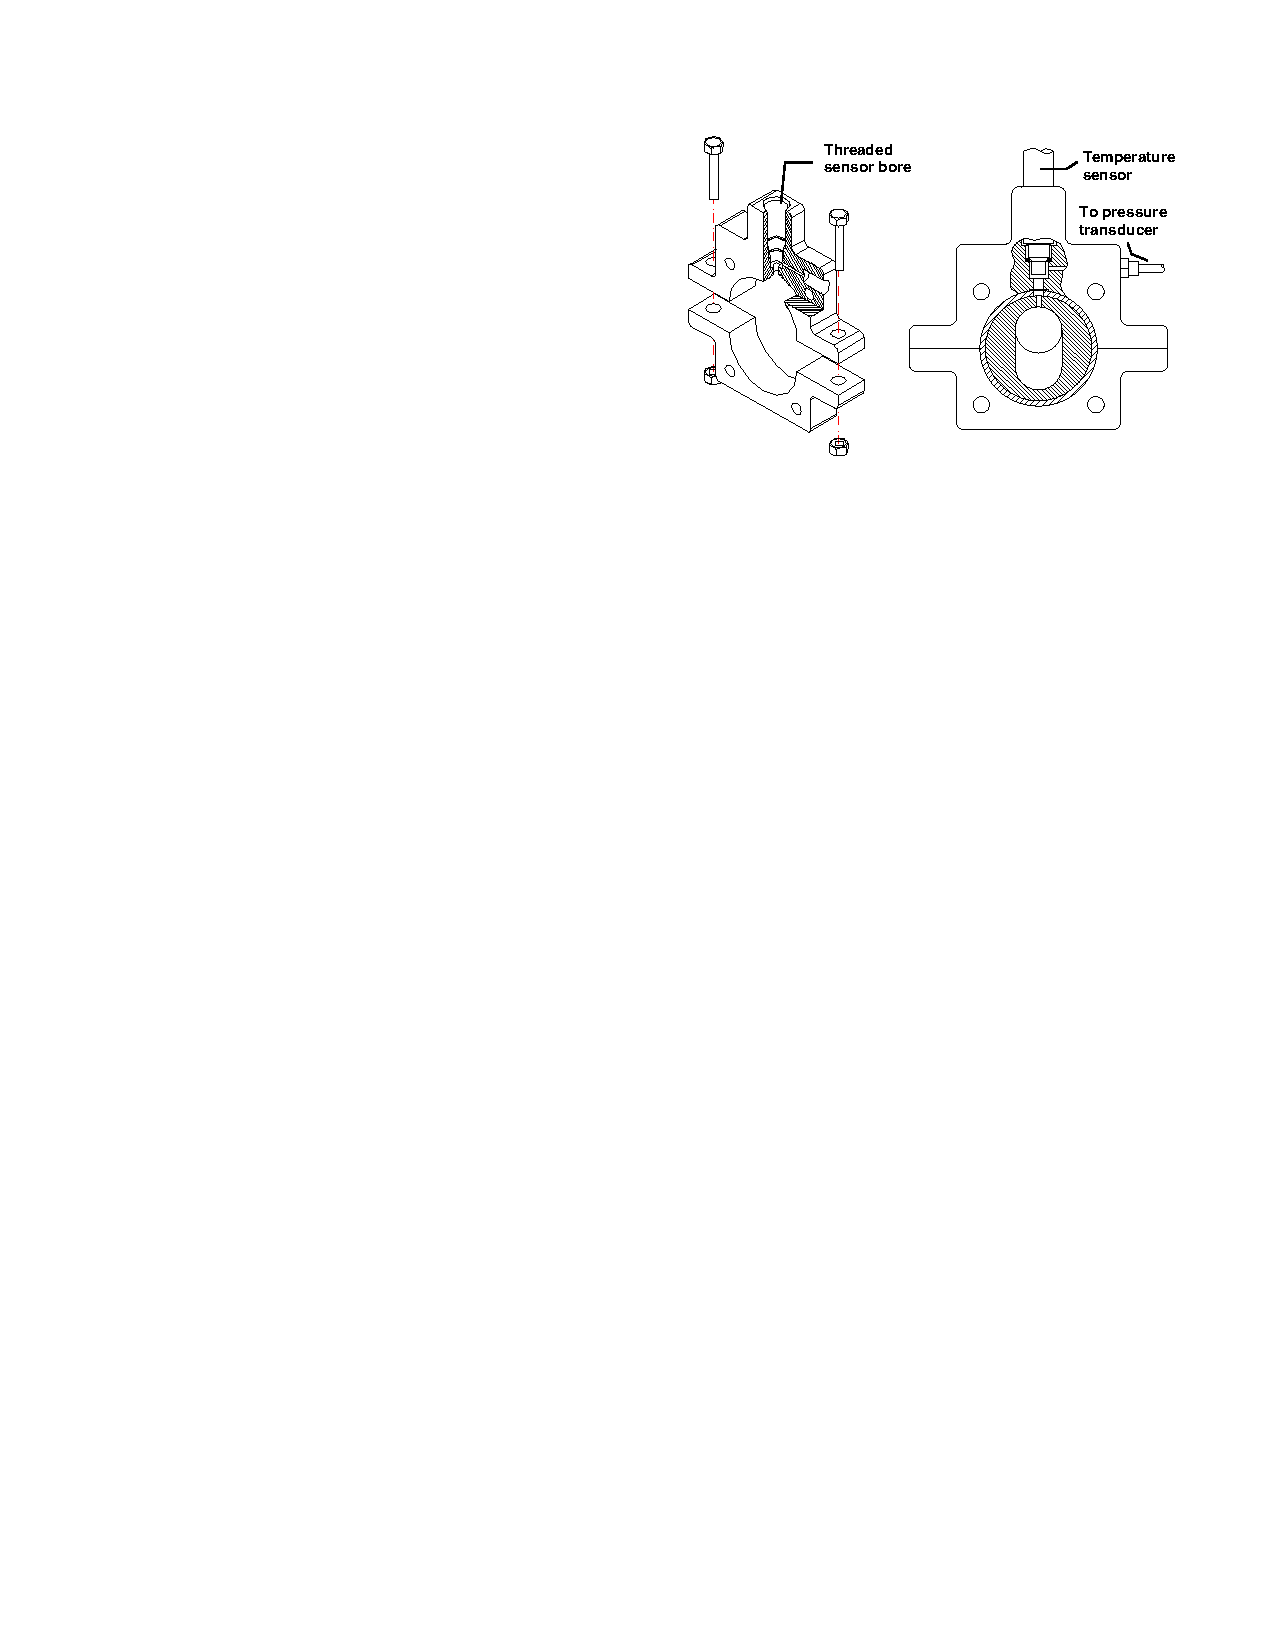
\includegraphics[scale=1,draft=false]{Accesorios_montaje_Martin-1999-426} 

\fuente{\textcite{Martin1999}}

\caption{Accesorios para el montaje de los sensores de presión y temperatura.}

\label{fig:Accesorios_montaje_Martin-1999-426}

\end{figure}

\begin{figure}

\centering
		
\includegraphics[scale=1,draft=false]{arreglo_sensores_Martin-1999-426} 

\fuente{\textcite{Martin1999}}

\caption{Arreglo de sensores a lo largo de la bomba.}

\label{fig:arreglo_sensores_Martin-1999-426}

\end{figure}

El circuito de prueba se ilustra en la Figura~\ref{fig:diagrama_circuito_Martin-1999-426}. Está compuesto por un compresor de aire, bomba de agua, tanque de separación, bomba de prueba en posición horizontal, válvula de alivio y válvula de control de presión a la descarga de la bomba de prueba. El circuito trabaja con agua y aire.

\begin{figure}

\centering
		
\includegraphics[scale=1,draft=false]{diagrama_circuito_Martin-1999-426} 

\fuente{\textcite{Martin1999}}

\caption{Diagrama del circuito experimental.}

\label{fig:diagrama_circuito_Martin-1999-426}

\end{figure}

Se realizaron estudios con flujo monofásico y bifásico. En la Figura~\ref{fig:distribucion_presion_Martin-1999-426}, se observa la distribución de presión a lo largo de la bomba para diferentes $\Delta P$ y 650 rpm con flujo monofásico. Se evidencia que para bajos gradientes de presión la máxima presión de la bomba no se encuentra en las últimas etapas de la bomba, sino hacia el centro  de la misma. Sin embargo, a medida que aumenta el $\Delta P$, la máxima presión de la bomba se desplaza hacia la descarga.


En la Figura~\ref{fig:distribucion_presion_bifasico_Martin-1999-426} están los resultados con flujo bifásico. Es notable el hecho de que casi todo el incremento de presión ocurre cerca de la descarga de la bomba, con muy poca importancia de la fracción de vacío de la mezcla bifásica. 


 
\begin{figure}

\centering
		
\includegraphics[scale=1,draft=false]{distribucion_presion_Martin-1999-426} 

\fuente{\textcite{Martin1999}}

\caption{Distribución de presión para varios $\Delta P$ con flujo monofásico.}

\label{fig:distribucion_presion_Martin-1999-426}

\end{figure}



\begin{figure}

\centering
		
\includegraphics[scale=1,draft=false]{distribucion_presion_bifasico_Martin-1999-426} 

\fuente{\textcite{Martin1999}}

\caption{Distribución de presión para varios $\Delta P$ con flujo bifásico.}

\label{fig:distribucion_presion_bifasico_Martin-1999-426}

\end{figure}


\begin{figure}

\centering
		
\includegraphics[scale=1,draft=false]{distribucion_temperatura_Martin-1999-426} 

\fuente{\textcite{Martin1999}}

\caption{Distribución de temperatura dentro de la bomba con flujo bifásico.}

\label{fig:distribucion_temperatura_Martin-1999-426}

\end{figure}


En la Figura~\ref{fig:distribucion_temperatura_Martin-1999-426} está la distribución de temperatura dentro de la bomba. \citeauthor{Martin1999} plantean que la distribución de temperatura en flujo bifásico podría ser causado por el relativo pobre desempeño de la conductividad térmica del elastómero. Atribuye el incremento de temperatura a la compresión del elastómero por el avance del rotor y, a su vez, a la fricción entre rotor y elastómero. Ambas acciones  ocurren de manera simultánea. La flexión cíclica del elastómero genera un calentamiento debido a la histéresis. Al incrementar la fracción de gas libre ocurre un aumento de la  temperatura  del estator. Mientras menos líquido hay dentro de la bomba, menos lubricación se tiene. 

\textcite{Olivet2002}

Los autores  estudiaron el desempeño de una BCP con estator metálico. La bomba tiene 3 etapas y se le colocaron 20 sensores de presión dispuestos como se puede observar en las Figuras 11 y 12. Se describen las curvas características y perfiles instantáneos de presión a lo largo de la bomba con flujo monofásico y bifásico. \citeauthor{Olivet2002} Demostraron que el escurrimiento con flujo bifásico es una función de la fracción de vacío, la presión diferencial y la velocidad de rotación de la bomba.

En este estudio 











